\documentclass{article}
\usepackage{amsmath, amssymb}
\usepackage{amsfonts}
\usepackage{amsthm}
\usepackage[algoruled]{algorithm2e}
\usepackage{titlesec}
\usepackage{graphicx}
\newcommand{\sectionbreak}{\clearpage}

\newcommand{\BigO}[1]{\ensuremath{\operatorname{O}\bigl(#1\bigr)}}
\renewcommand{\vec}[1]{\mathbf{#1}}

\newtheorem{example}{Example}[section]
\newtheorem{thm}{Theorem}[section]
\newtheorem{lem}{Lemma}[section]
\newtheorem{definition}{Definition}[section]
\newtheorem{cor}{Corollary}[section]

\begin{document}

%%%%%%%%%%%%%%%%%%%%%%%%%%%%%%%%%%%%%%%%%%%%%%%%

\begin{algorithm}[H]
 \SetLine % For v3.9
 %\SetAlgoLined % For previous releases [?]
 \KwData{A Set \(S\) of \(\lvert S \rvert = n\) items, \(\mu\) of which are actually defective in expectation, a probability vector \( \vec{p}^{\left(n\right)} \) describing each item's independent probability of being defective, and a cutoff \(\theta\)}
 \KwResult{The set of defective items}
 Discard items with \(p_i \leq \theta\)
 \\
 Sort the remaining items into \(B\) bins, collecting items together with \(p_i \in \left[1/2C^r,1/2C^{r-1}\right)\) in bin \(r\).
 \\
 Sort the items in each bin into sets s.t. the (normalised) probability of each set is less than \(1/2\).
 \\
 Test each set in turn
 \\
   	\If{The test is positive}{Arrange the items in the set on a Shannon-Fano/Huffman Tree and search the set for all the defectives it contains}

 \caption{Algorithm for the non-iid group testing problem}
\end{algorithm}

\section{Results}
The performance of the above algorithm (in terms of the sample complexity) were analysed by simulating 500 items, with a mean number of defectives equal to 8. I.e. \(N = 500\) and \(\mu = 8\). 

The probability distribution \(\vec{p}\) was generated by a Dirichlet distribution. We cannot simply choose a set of random numbers and normalise by the sum. Consider the case of two random numbers, \(\left(x,y\right)\), distributed uniformly on the square \(\left[0,1\right]^2\). Normalising by the sum \(\left(x+y\right)\) projects the point \(\left(x,y\right)\) onto the line \(x+y=1\) and so favours points closer to \((0.5,0.5)\) than the endpoints. The Dirichlet distribution avoids this by generating points directly on the simplex.

We then chose values of the cutoff parameter \(\theta\) from 0.0001 to 0.01, and for each \(\theta_i\) simulated the algorithm 1000 times. We plot the empirical distribution of tests, varying theta as well as the uniformity/concentration of the probability distribution (via the parameter \(\alpha\) of the Dirichlet distribution). We also plot, the theoretical lower and upper bounds on the number of Tests required for successful recovery alongside the empirical number tests (all as a function of \(\theta\)).

\begin{figure}[h]
\centering
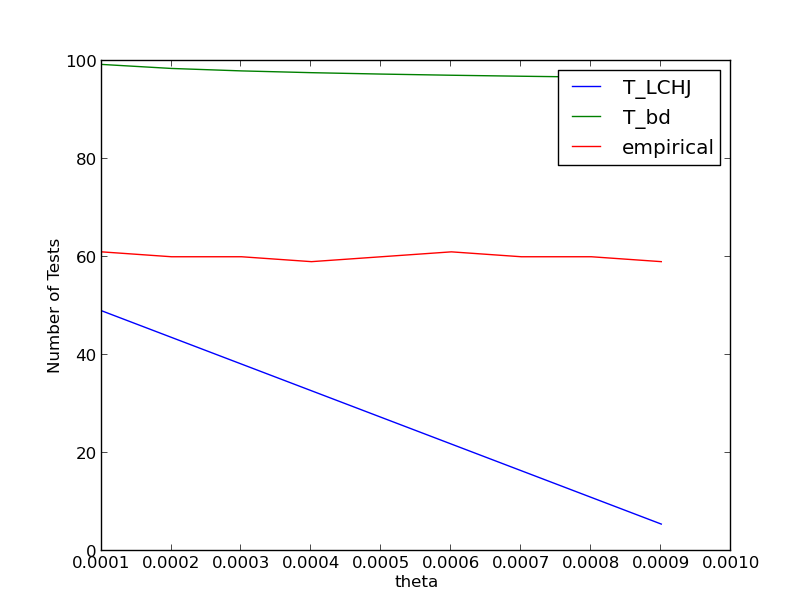
\includegraphics[width=0.7\textwidth]{ubvslb.png}
\caption{Theoretical lower and upper bounds and empirical Test frequencies as functions of \(\theta\)}
\label{ubvslb}
\end{figure}

Note that the Upper bound is not optimal and there still is some room for improvement. Note also that the lower bound degrades with \(\theta_i\). 

\begin{figure}[h]
\centering
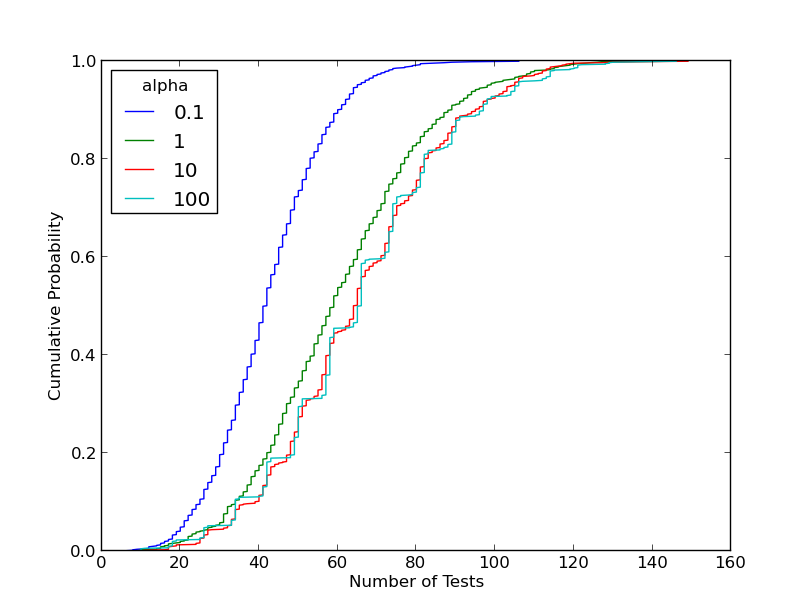
\includegraphics[width=0.7\textwidth]{variousalpha.png}
\caption{Cumulative distribution curves of the modified Hwang algorithm with fixed \(\theta = 0.0001\) and \(\alpha\) varying }
\label{testsvsalpha}
\end{figure}

\begin{figure}[h]
\centering
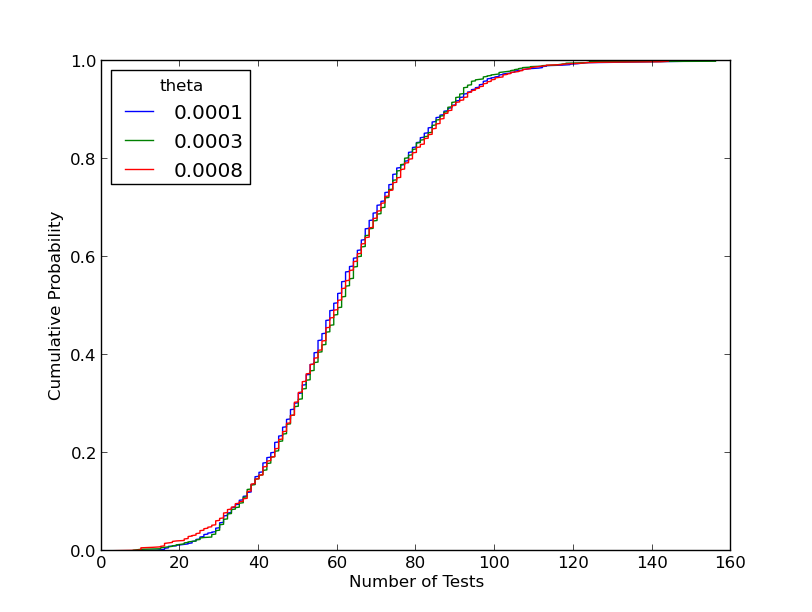
\includegraphics[width=0.7\textwidth]{nicegraphlaminar.png}
\caption{Cumulative distribution curves for fixed \(\alpha = 1\) and varying \(\theta\)}
\label{testsvstheta}
\end{figure}

Figures (\ref{testsvsalpha}) and (\ref{testsvstheta}) show that the performance is relatively insensitive to the cut-off \(\theta\), and more sensitive to the uniformity (or otherwise) of the probability distribution \(\vec{p}\). Heuristically, this is for because distributions which are highly concentrated on a few items algorithms can make substantial savings on the testing budget by testing those highly likely items first (which is captured in the bin structure of the above algorithm). 

The insensitivity to the cutoff \(\theta\) is due to items below \(\theta\) being overwhelmingly unlikely to be defective - which for small \(\theta\) means that few items (relative to the size of the problem) get discarded.

\end{document}